\begin{align*}
    \polynomialQ{2}{N}{0} &= 0 \\
    \polynomialQ{2}{N}{1} &= 1 \\
    \polynomialQ{2}{N}{2} &= 30N^2 - 60N + 32 \\
    \polynomialQ{2}{N}{3} &= 150N^2 - 540N + 513 \\
    \polynomialQ{2}{N}{4} &= 420N^2 - 2160N + 2944 \\
    \polynomialQ{2}{N}{5} &= 900N^2 - 6000N + 10625 \\
    \polynomialQ{2}{N}{6} &= 1650N^2 - 13500N + 29376 \\
    \polynomialQ{2}{N}{7} &= 2730N^2 - 26460N + 68257 \\
    \polynomialQ{2}{N}{8} &= 4200N^2 - 47040N + 140288 \\
    \polynomialQ{2}{N}{9} &= 6120N^2 - 77760N + 263169 \\
    \polynomialQ{2}{N}{10} &= 8550N^2 - 121500N + 460000 \\
    \polynomialQ{2}{N}{11} &= 11550N^2 - 181500N + 760001 \\
    \polynomialQ{2}{N}{12} &= 15180N^2 - 261360N + 1199232 \\
    \polynomialQ{2}{N}{13} &= 19500N^2 - 365040N + 1821313 \\
    \polynomialQ{2}{N}{14} &= 24570N^2 - 496860N + 2678144 \\
    \polynomialQ{2}{N}{15} &= 30450N^2 - 661500N + 3830625 \\
    \polynomialQ{2}{N}{16} &= 37200N^2 - 864000N + 5349376 \\
    \polynomialQ{2}{N}{17} &= 44880N^2 - 1109760N + 7315457 \\
    \polynomialQ{2}{N}{18} &= 53550N^2 - 1404540N + 9821088 \\
    \polynomialQ{2}{N}{19} &= 63270N^2 - 1754460N + 12970369 \\
    \polynomialQ{2}{N}{20} &= 74100N^2 - 2166000N + 16880000
\end{align*}
\begin{figure}[H]
    \centering
    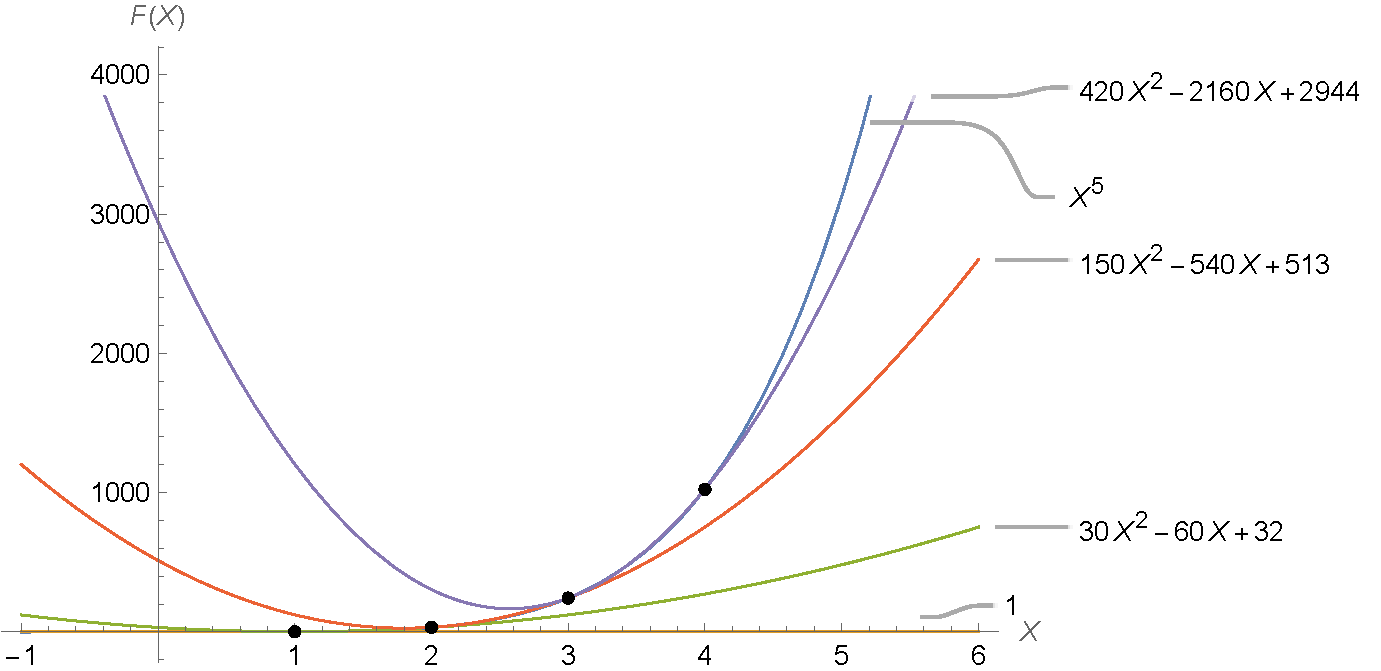
\includegraphics[width=1\textwidth]{sections/images/04_fifth_power_with_q_1_n_k}
    ~\caption{Polynomials P(2, n, k)}\label{fig:figure4}
\end{figure}
